	\documentclass[runningheads, envcountsame, a4paper]{llncs}

\usepackage{amsmath}
\usepackage{amssymb}
\usepackage{graphicx}
\usepackage{makeidx}  
\usepackage{enumerate}
\usepackage{textcomp}         
\usepackage{verbatim}
\usepackage[caption=false]{subfig}
\usepackage{cite}
\usepackage{multirow}

\begin{document}
\mainmatter           
\title{Constructing Parsimonious Hybridization Networks from Multiple Phylogenetic Trees Using a SAT-solver}
\titlerunning{ } 
\toctitle{ }

\author{Vladimir Ulyantsev \and Mikhail Melnik}
\authorrunning{V. Ulyantsev, M. Melnik} 
\tocauthor{Vladimir~Ulyantsev, Mikhail~Melnik}
\institute{ITMO University, Saint Petersburg, Russia \\
\email{$\{$ulyantsev,melnik$\}$@rain.ifmo.ru}}

\maketitle
\setcounter{footnote}{0}

\begin{abstract}
  We present an exact algorithm for constructing minimal hybridization networks from multiple trees 
  which is based on reducing 
  the problem to the Boolean satisfiability problem. The main idea of our algorithm is to iterate over
  possible hybridization numbers and to construct for each of them a Boolean formula that is satisfiable iff there
  exists a network with such hybridization number. The proposed algorithm is implemented in a software tool PhyloSAT.
  The experimental evaluation of our algorithm on biological data shows that our method is as far as we know the 
  fastest exact algorithm for the minimal hybridization network construction problem.

  \keywords{Phylogenetic networks, Boolean satisfiability, SAT, bioinformatics, genetics}
\end{abstract}

\section{Introduction}

A phylogenetic network is a powerful model for reticulate
evolutionary processes (such as horizontal gene transfer and hybrid specification).
Briefly, a phylogenetic network is a directed acyclic graph which has
nodes (called reticulation nodes) with more than one incoming edge. Phylogenetic
networks have been studied by several researchers~\cite{huson2010phylogenetic, morrison2011introduction, 
nakhleh2011evolutionary}. There are several formulations of phylogenetic network
construction problem with various modelling assumptions and different types of input data. 
In this paper we focus on the specific type of phylogenetic networks called hybridization
networks~\cite{semple2006hybridization, chen2010hybridnet}.

As input data for hybridization network construction we consider a set of gene trees on the same set of taxa.
Each gene tree models the evolutionary history of some gene. 
Due to reticulate evolutionary events, these trees can have different topologies.
The aim is to construct a hybridization network containing the smallest possible number of 
reticulation nodes and displaying each of the input trees. 

Most of the algorithms for hybridization network construction are heuristic~\cite{wu2013algorithm, park2012murpar} 
and usually deal with only two trees.
However, the exact algorithm PIRN$_\mathrm{C}$ has been introduced recently~\cite{wu2013algorithm}, which is able to process more than two input trees.

In this paper we introduce a new approach for exact parsimonious
hybridization network construction from multiple input trees based on satisfiability (SAT) solvers.
The SAT problem is known to be NP-complete~\cite{bordewich2007computing}, but state-of-the-art SAT-solvers running on modern hardware 
are able to solve SAT instances having tens of thousands of variables and hundreds of thousands of clauses in several minutes.

SAT-solver based algorithms have been successfully applied to efficiently calculate evolutionary tree measures~\cite{bonet2009efficiently}
as well as to solve problems in other domains such as
finite-state machine induction~\cite{heule2010exact}, software verification~\cite{biere2003bounded}.

The general outline of our approach is to convert an instance of hybridization network construction 
problem to an instance of the SAT problem (a Boolean formula), solve it using a SAT-solver and then if the
solution exists convert 
the satisfying assignment into the hybridization network.
Our approach leads to an exact algorithm that outperforms PIRN$\mathrm{_C}$ on our tests.

The paper is structured as follows. Section 2 gives the formal definitions, Section 3 describes the Boolean formula
construction process and Section 4 gives the experimental results. The paper is concluded in Section 5.

\section{Definitions and Background}

\begin{figure}[t]
  \centering
  \includegraphics[width=1.4in]{pics/inp1.eps}
  ~~~
  \includegraphics[width=1.4in]{pics/inp2.eps}
  ~~~
  \includegraphics[width=1.4in]{pics/inp3.eps}
  \caption{Example of three gene trees over the set of taxa \{a, b, c, d, e\}.}
  \label{input-example}
\end{figure}

\begin{figure}[t]
  \centering
  \includegraphics[width=1.4in]{pics/ans.eps}
  ~~~~~~
  \includegraphics[width=1.4in]{pics/ans3.eps}
  \caption{Possible hybridization networks for the trees from Fig.~\ref{input-example} with two and three hybridization events respectively. Reticulation nodes are shown as boxes.}
  \label{network-example}
\end{figure}

We define a \emph{phylogenetic tree} as a leaf-labelled tree constructed over a set of taxa. 
Throughout this paper we assume that trees are rooted and binary.

For any node $v$ let $d^-(v)$ be the in-degree of $v$ and $d^+(v)$ be the out-degree of $v$.
A \emph{hybridization network} on a set of taxa $X$ is a directed acyclic graph 
with a single root $\rho$ and leaves bijectively mapped to the set of taxa $X$. If $d^-(v) > 1$ then 
node $v$ is called a \emph{reticulation node}. In this paper we assume that $d^-(v) = 2$ and $d^+(v) = 1$ is true for every reticulation node $v$.
We make this assumption by noting that we can convert a reticulation node with in-degree 
of three or more to a sequence of reticulation nodes with in-degrees of two~\cite{wu2010close}. Other nodes are regular 
tree nodes.

Every hybridization network $N$ can be reduced to a tree. To do this we firstly keep only one of the incoming edges for each reticulation node in $N$. 
And secondly we contract edges to remove any node $v$ such that $d^-(v) = d^+(v) = 1$. With these two steps we reduce the network $N$ 
to the tree $T'$.

We say that hybridization network $N$ \emph{displays} phylogenetic tree $T$ 
if we can choose the edges of reticulation nodes in such a way that after edge-contraction the obtained tree $T'$ will be 
isomorphic to $T$. In Figure~\ref{network-example} each of the three trees from Figure~\ref{input-example} is displayed in both hybridization networks.

A \emph{hybridization number} of network $N$ with root $\rho$ is commonly defined as $h(N) = \sum\limits_{v \ne \rho} (d^-(v) - 1)$.
Note that under our assumptions $h(N)$ simply equals the number of reticulation nodes.

Suppose we are given a set of $K$ phylogenetic trees $T_1, T_2, \dots, T_k$ over the same set of taxa. The \emph{minimal 
hybridization network} for that set of trees is a network $N\mathrm{_{min}}$ that displays each tree and has the smallest 
hybridization number possible. Note that there can be several networks with equal hybridization number.

\emph{The most parsimonious hybridization network problem} is defined as follows:
given a set of phylogenetic trees $T_1, T_2, \dots, T_k$ over the same set of taxa, construct the minimal hybridization 
network for this set of trees.

It has been shown that even for the case of $k=2$ the construction of such a network is an NP-complete problem 
\cite {bordewich2007computing}. As far as we know there exists only one algorithm for the construction of the most 
parsimonious hybridization network~\cite{wu2013algorithm}.

\section{Algorithm}

The main idea of our algorithm is to iterate over possible values of the hybridization number and to construct and solve a Boolean 
formula that represents a hybridization network with this hybridization number.
We implemented our algorithm in a software tool PhyloSAT which is available for download at GitHub\footnote{\url{https://github.com/ctlab/PhyloSAT}}.

\subsection{Pre-processing}

Before the actual Boolean formula encoding we modify the input and split it into several tasks to reduce the size 
and the complexity of the problem. We do this according to the rules from~\cite{bonet2009efficiently}. To define these 
rules we first need to define the term \emph{cluster}: a set of taxa $A$ is a cluster in trees $T_1, T_2, \dots, T_k$ if there 
exists a node in each tree with the set of leaves of its subtree equal to the set $A$. The reduction rules are as follows:

\begin{enumerate}

\item \textbf{Subtree reduction rule}:
replace every subtree which is present in all input trees with a leaf with a new label.

\item \textbf{Cluster reduction rule}:
for each cluster $A$ replace the subtrees containing it with a leaf with a new label and add a new task for processing 
which consists of deleted subtrees $T'_1, T'_2, \dots, T'_k$ with leaf set $A$.

\end{enumerate}

After we split the task into a set of simpler tasks, we add a dummy root to each tree of each task along with 
the new dummy leaf for tree consistency. Figure~\ref{dummy-example} illustrates the procedure. 
This is done to ensure that all the trees in the input share a common root. 
This dummy root will be deleted on the post-processing stage. At this stage we have a set of tasks that will be solved 
separately and then their results will be merged at the post-processing stage.

\begin{figure}[t]
  \centering
  \begin{minipage}[b]{0.39\linewidth}
    \includegraphics[width=0.7in]{pics/inp_dummy.eps}
    \centering{\\ (a) Simple tree}
  \end{minipage}
  \hfill
  \begin{minipage}[b]{0.59\linewidth}
    \includegraphics[width=0.7in]{pics/ans_dummy.eps}
    \centering{\\ (b) Simple tree with dummy root attached}
  \end{minipage}
  \caption{An illustration of an attachment of the dummy root to the tree.}
  \label{dummy-example}
\end{figure}

\subsection{Search of the minimal hybridization number}

To solve a subtask we need to find the lowest hybridization number $k$ such that there exists a hybridization 
network with this hybridization number. To do this we use downwards search, i.e. we iterate through possible values of $k$ starting from the highest 
and construct a Boolean formula corresponding to the current $k$. 
We decrease $k$ until the solver cannot satisfy the formula, and this means that the previous value of $k$ was the 
lowest possible.

There are other strategies of searching the minimal value of $k$. For example, we can start from 
zero and increase the value of $k$ until the solver will be able to satisfy the formula, or we can use binary search. 
The results of the binary search were close to the ones of downwards method, 
but in some cases, when the binary search tried to satisfy formulae with values of $k$ less than minimal possible hybridization number, 
its results were also poor. 
This can be explained by an experimental observation that it is usually easier for the solver to produce an answer if the formula is satisfiable than if it is not. 
In case of an unsatisfiable formula the solver must check every possible answer to ensure that there is no solution; this is not needed if the 
formula is satisfiable. Because of this the results of the upwards search were poor. An obvious method 
for reducing the search time is to limit the range of possible values of $k$ by using different heuristics to find close upper and lower bounds for $k$. 
Possible candidates are PIRN$\mathrm{_{CH}}$~\cite{wu2013algorithm}, RIATA-HGT~\cite{nakhleh2005riata} and MURPAR~\cite{park2012murpar}. We do not consider such optimizations in this paper.

\subsection{Encoding the Boolean formula}

Having a set of trees $T$ over a set of taxa $A$ and a fixed hybridization number $k$, we will construct a Boolean formula 
which is satisfiable iff there exists a hybridization network that displays each tree in $T$ and its hybridization 
number equals to $k$. To do this we first notice that a network over the set of taxa of size $n$ with hybridization number 
$k$ will have $2 (n + k) - 1$ nodes. As we add a dummy root and a dummy leaf, we finally have $2 (n + k) + 1$ nodes, 
$k$ of which are reticulation nodes, $n + 1$ are leaves and others are usual tree nodes.

We enumerate all the nodes in such a way 
that leaves are numbered in range $[0,n]$, regular nodes have numbers in range $[n + 1,2n + k]$ and all reticulation nodes have numbers 
in range $[2n + k + 1, 2(n + k)]$. We also assume that the number of any leaf or regular node is less than the number of its parent. This is done to 
avoid consideration of isomorphic networks during SAT solving. Such enumeration allows us to define the following sets of nodes for each node 
$v$: $PC(v)$ is the set of possible children of $v$, $PP(v)$ is the set of possible parents of $v$ and $PU(v)$ is the set of possible ancestors of $v$. Also let $R$ be the set of reticulation nodes, $L$ be the set of leaves and $V$ be the set of regular nodes. 
Now we will describe variables and clauses required to construct the Boolean formula.

\subsubsection{Network structure encoding.} 

First, we encode the structure of the network. We introduce the following literals. 

\begin{enumerate}

\item $l_{v,u}$ and $r_{v,u}$ for each $v \in V, u \in PC(v)$ : 
$l_{v,u}$ (or $r_{v,u}$) is true iff regular node $v$ has node $u$ as its left (right) child.

\item $p_{v,u}$  for each $v \in L \cup V \backslash \{\rho\}, u \in PP(v)$ :
$p_{v,u}$ is true iff $u$ is the parent of a regular node $v$.

\item $p^l_{v,u}$ and $p^r_{v,u}$ for each $v \in R, u \in PP(v)$ :
$p^l_{v,u}$ (or $p^r_{v,u}$) is true iff $u$ is the left (right) parent of a reticulation node $v$.

\item $c_{v,u}$ for each $v \in R, u \in PC(v)$ :
$c_{v,u}$ is true iff $u$ is a child of a reticulation node $v$.

\end{enumerate}

This takes $O((n + k)^2)$ literals for specifying the network structure, and by noticing that $k < n$ we have $O(n^2)$ literals.

To encode the uniqueness of parents and children we tried to use an obvious pairwise encoding that requires 
$O(n^2)$ clauses for each node as well as more efficient Bimander encoding \cite{nguyenefficient}. However the Bimander encoding gave no speed boost because of the existence of other constraints that require $O(n^2)$ clauses per node.
Thus we will describe the pairwise encoding for simplicity.
For example consider parent variables. We state that a node can have at least one parent and at most one parent. For parents of the regular node $v$ this can be expressed 
in the following way: 
$$\left(\bigvee\limits_{u \in PP(v)} p_{v,u}\right) \wedge \left(\bigwedge\limits_{i, j \in PP(v);i < j} \left(p_{v,i} \rightarrow \neg p_{v,j}\right)\right).$$

Using this pattern, we add the uniqueness constraints for literals $l$, $r$, $p$, $p^l$, $p^r$ and $c$. 
These clauses are defined in sections 1--4 of Table~\ref{network-table}. 
We also add constraints to order the number of children of regular nodes and parents of reticulation nodes.
They are listed in section 5 of Table~\ref{network-table}.

\begin{table}[t]
\centering
\caption{Clauses for network structure encoding.}
\begin{tabular}{l | l | l}
  Number & Clause & Range \\
  
  \hline
  1.1 &
  $p_{v,u_1} \vee \dots \vee p_{v,u_k}$ &
  $v \in V; u_1 \dots u_k \in PP(v)$
  \\
  1.2 &
  $p_{v,u} \rightarrow \neg p_{v,w}$ &
  $v \in V; u, w \in PP(v)$
  \\
  
  \hline
  2.1 &
  $l_{v,u_1} \vee \dots \vee l_{v,u_k}$ &
  $v \in V; u_1 \dots u_k \in PC(v)$
  \\
  2.2 &
  $l_{v,u} \rightarrow \neg l_{v,w}$ &
  $v \in V; u, w \in PC(v)$
  \\
  2.3 &
  $r_{v,u_1} \vee \dots \vee r_{v,u_k}$ &
  $v \in V; u_1 \dots u_k \in PC(v)$
  \\
  2.4 &
  $r_{v,u} \rightarrow \neg r_{v,w}$ &
  $v \in V; u, w \in PC(v)$
  \\
  
  \hline
  3.1 &
  $c_{v,u_1} \vee \dots \vee c_{v,u_k}$ &
  $v \in R; u_1 \dots u_k \in PC(v)$
  \\
  3.2 &
  $c_{v,u} \rightarrow \neg c_{v,w}$ &
  $v \in R; u, w \in PC(v)$
  \\
  
  \hline
  4.1 &
  $p^l_{v,u_1} \vee \dots \vee p^l_{v,u_k}$ &
  $v \in R; u_1 \dots u_k \in PP(v)$
  \\
  4.2 &
  $p^l_{v,u} \rightarrow \neg p^l_{v,w}$ &
  $v \in R; u, w \in PP(v)$
  \\
  4.3 &
  $p^r_{v,u_1} \vee \dots \vee p^r_{v,u_k}$ &
  $v \in R; u_1 \dots u_k \in PP(v)$
  \\
  4.4 &
  $p^r_{v,u} \rightarrow \neg p^r_{v,w}$ &
  $v \in R; u, w \in PP(v)$
  \\

  \hline
  5.1 &
  $l_{v,u} \rightarrow \neg r_{v,w}$ &
  $v \in V; u, w \in PC(v): u \geq w$
  \\
  5.2 &
  $p^l_{v,u} \rightarrow \neg p^r_{v,w}$ &
  $v \in R; u, w \in PP(v) : u \geq w$
  \\
  
  \hline
  6.1 &
  $l_{v,u} \rightarrow p_{u,v}$ &
  \multirow{3}{*}{$v \in V; u \in V \cap PC(v)$}
  \\
  6.2 &
  $r_{v,u} \rightarrow p_{u,v}$ &
  %$v \in V; u \in V \cap PC(v)$
  \\
  6.3 &
  $p_{u,v} \rightarrow (l_{v,u} \vee r_{v,u})$ &
  %$v \in V; u \in V \cap PC(v)$
  \\
  
  \hline
  7.1 &
  $l_{v,u} \rightarrow (p^l_{u,v} \vee p^r_{u,v})$ &
  $v \in V; u \in R \cap PC(v)$
  \\
  7.2 &
  $r_{v,u} \rightarrow (p^l_{u,v} \vee p^r_{u,v})$ &
  $v \in V; u \in R \cap PC(v)$
  \\
  7.3 &
  $p^l_{u,v} \rightarrow (l_{v,u} \vee r_{v,u})$ &
  $v \in V; u \in R \cap PC(v)$
  \\
  7.4 &
  $p^r_{u,v} \rightarrow (l_{v,u} \vee r_{v,u})$ &
  $v \in V; u \in R \cap PC(v)$
  \\
  
  \hline 
  8.1 &
  $c_{v,u} \rightarrow p_{u,v}$ &
  $v \in R; u \in V \cap PC(v)$
  \\
  8.2 &
  $p_{u,v} \rightarrow c_{v,u}$ &
  $v \in R; u \in V \cap PC(v)$
  \\
  
  \hline
  9.1 &
  $c_{v,u} \rightarrow (p^l_{u,v} \vee p^r_{u,v})$ &
  $v \in R; u \in R \cap PC(v)$
  \\
  9.2 &
  $p^l_{u,v} \rightarrow c_{v,u}$ &
  $v \in R; u \in R \cap PC(v)$
  \\
  9.3 &
  $p^r_{u,v} \rightarrow c_{v,u}$ &
  $v \in R; u \in R \cap PC(v)$
  \\
  
  \hline
  10.1 &
  $c_{v,u} \rightarrow \neg p^l_{v,w}$ &
  $v \in R; u \in PC(v); w \in PP(v): u \geq w$
  \\
  10.2 &
  $c_{v,u} \rightarrow \neg p^r_{v,w}$ &
  $v \in R; u \in PC(v); w \in PP(v): u \geq w$
  \\
  
\end{tabular}
\label{network-table}
\end{table}

A network is consistent if for every pair of nodes the parent relation implies the child relation and vice versa. Thus we add constraints that connect parent literals with children literals for all the types of nodes. See sections 6--9 of Table~\ref{network-table} for these clauses.
The last step of the network construction is to deal with the enumeration around reticulation nodes. To do this, we add constraints to fix 
relative numbers of children and parents of reticulation nodes. They are defined in section 10 of Table~\ref{network-table}.

Since we need $O(n^2)$ clauses for each node to represent the uniqueness of its parents and children 
and $O(n)$ clauses for each node to represent the parents-children relation, we finally get $O(n^3)$ clauses in total 
to represent the network structure.

\subsubsection{Mapping trees to the network.}

To express that the network contains all the input trees we add literals that represent the mapping of the tree nodes to 
the network nodes.

\begin{enumerate}

\item $x_{t,v_t,v}$ for each $t \in T, v_t \in V(t), v \in V$ :
$x_{t,s,v}$ is true iff regular node $v$ represents node $v_t$ from tree $t$, i.e. $x$ literals represent injective 
mapping of network nodes to tree nodes. An example of such mapping is shown in Figure~\ref{mapping-example}.
Note that leaves of the trees are bijectively mapped to leaves of the network thus there is no need to introduce $x$ variables for them.

\item $d_{t,v}$ for each $t \in T, v \in R$ :
$d_{t,v}$ is true iff the left parent edge of reticulation node $v$ is used to display tree $t$,
 i.e. it specifies direction of necessary parent to display current tree.

\item $u^r_{t,v}$ for each $t \in T, v \in R$ :
$u^r_{t,v}$ is true iff the child of reticulation node $v$ is used to display tree $t$.

\item $u_{t,v}$ for each $t \in T, v \in V$ :
$u_{t,v}$ is true iff regular node $v$ is used to display tree $t$.

\item $a_{t,v,u}$ for each $t \in T, v \in V, u \in PU(v)$ :
$a_{t,v,u}$ is true iff regular node $u$ is an ancestor of node $v$ and node $u$ corresponds to such node $u_t$ 
from tree $t$ that all the edges on the path from $u$ to $v$ are contracted to a single edge of tree $t$, i.e. node
$u$ is the first node on the path from $v$ to the root that is mapped to some node in tree $t$.
We will say that node $u$ is the direct parent of node $v$ considering tree $t$. Note that node $v$ is not necessary present in tree $t$.
In Figure~\ref{mapping-example} node $u$ is the parent of all the nodes starting from node $v$ considering tree $t$.

\end{enumerate}

\begin{figure}[t]
  \centering
  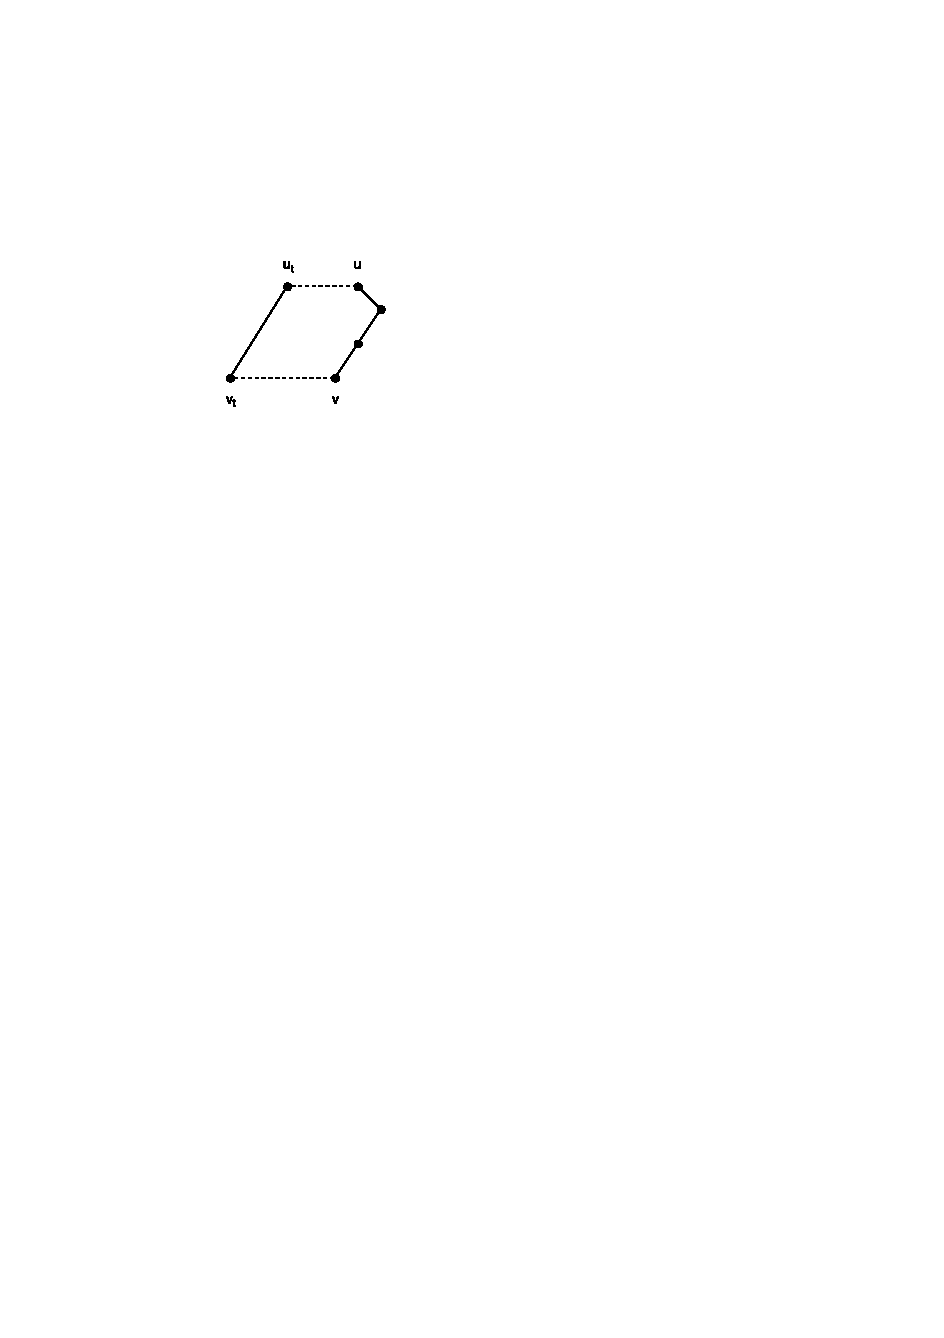
\includegraphics[width=1in]{pics/up_var.eps}
  \caption{An illustration of a piece of mapping of the nodes from the tree (on the left) to the nodes from the network (on the right). 
  Nodes that are injectively mapped are connected by a dotted line. When displaying the tree all the edges in the path from $u$ to $v$
  will be contracted to the single edge form $u_t$ to $v_t$.}
  \label{mapping-example}
\end{figure}

We have extra $O(tn^2)$ literals to match input trees to the network. Hence, we have $O(tn^2)$ literals in total.

We specify constraints for relations between network nodes and tree nodes. 
First, we define at-least-one and at-most-one constraints for literals $x$ and $a$. Note that in case 
of $x$ literals we have a restriction that at most one node from the tree corresponds to the network node, and that at 
most one node from the network corresponds to the tree node. These clauses are defined in sections 1--2 of Table~\ref{mapping-table}.
Because of dummy roots we know that roots of input trees 
are mapped to the root of the network so we have $x_{t,\rho_t,\rho}$ set to true for every tree. Also 
note that $x_{t,v_t,v}$ implies $u_{t,v}$ by definition. See section 3 of Table~\ref{mapping-table} for these clauses.

\begin{table}[t]
\centering
\caption{Clauses for the mapping of the tree nodes to the network nodes.}
\begin{tabular}{l | l | l}
  & Clause & Range \\
  
  \hline
  1.1 &
  $a_{t,v,u_1} \vee \dots \vee a_{t,v,u_k}$ &
  $v \in V \cup L \cup R; u_1 \dots u_k \in PU(v)$
  \\
  1.2 &
  $a_{t,v,u} \rightarrow \neg a_{t,v,w}$ &
  $v \in V \cup L \cup R; u, w \in PU(v)$
  \\
  
  \hline
  2.1 &
  $x_{t,t_v,v_1} \vee \dots \vee x_{t,t_v,v_k}$ &
  $t \in T; t_v \in V(t); v_1 \dots v_k \in V$
  \\
  2.2 &
  $x_{t,t_v,v} \rightarrow \neg x_{t,t_v,w}$ &
  $t \in T; t_v \in V(t); v, w \in V$
  \\
  2.3 &
  $x_{t,t_v,v} \rightarrow \neg x_{t,t_w,v}$ &
  $t \in T; t_v, t_w \in V(t); v \in V$
  \\

  \hline
  3.1 &
  $x_{t,v_t,v} \rightarrow u_{t,v}$ &
  $t \in T; v \in V; v_t \in V(t)$  
  \\
  3.2 &
  $x_{t,\rho_t,\rho}$ &
  $t \in T; \rho_t = \rho(t)$
  \\
  
  \hline
  4.1 &
  $x_{t,u_t,u} \rightarrow a_{t,v,u}$ &
  $t \in T; v \in L; u \in PP(v); u_t \in V(t)$
  \\
  
  4.2 &
  $(x_{t,v_t,v} \wedge x_{t,u_t,u}) \rightarrow a_{t,v,u}$ &
  $t \in T; v \in V; u \in PP(v); v_t \in V(t): u_t = p(v_t)$
  \\
  
  4.3 &
  $(x_{t,v_t,v} \wedge a_{t,v,u}) \rightarrow x_{t,u_t,u}$ &
  $t \in T; v \in V; u \in PP(v); v_t \in V(t): u_t = p(v_t)$
  \\

  4.4 &
  $x_{t,v_t,v} \rightarrow \neg x_{t,u_t,u}$ &
  $t \in T; v \in V; u \in V; v_t \in V(t); u_t = p(v_t): u < v$
  \\
  
  \hline
  5.1 &
  $\neg x_{t,v_t,v}$ &
  $t \in T; v \in V; v_t \in V(t): v_t < \mathrm{size}(\mathrm{subtree}(v_t))$
  \\
  
  5.2 &
  $\neg x_{t,v_t,v}$ &
  $t \in T; v \in V; v_t \in V(t): v_t > \mathrm{size}(t) - \mathrm{depth}(v_t)$
  \\
  
  5.3 &
  $\neg x_{t,v_t,v} \vee \neg x_{t',v_{t'},v}$ &
  $t, t' \in T; v \in V; v_t \in V(t); v_{t'} \in V(t') :$
  \\
  & & subtrees of $t$ and $t'$ have disjoint sets of taxa
  
\end{tabular}
\label{mapping-table}
\end{table}

Furthermore, if we know that node $v$ is a leaf and its parent $u$ corresponds to node $u_t$ from tree $t$, 
then we can conclude that $a_{t,v,u}$ is true i.e. $u$ is the direct parent of $v$ in tree $t$. The same observation 
can be done for non-leaves, i.e. if we know that $v$ corresponds to $v_t$ and another node $u$ corresponds to $u_t$ 
and $u_t$ is parent of $v_t$ then $u$ is the direct parent of $v$ considering tree $t$. On the other hand if we know 
that $v$ corresponds to $v_t$ and we know that $u$ is the direct parent of $v$ considering tree $t$, then $u$ should 
correspond to parent of $v_t$. We also should take care of enumeration, so we add a constraint stating that if node 
$u_t$ is the parent of the node $v_t$, then the number of the corresponding node $u$ should be greater than the one of 
the node $v$, i.e. $x_{t,v_t,v} \rightarrow \neg x_{t,u_t,u}$ for each $u$ and $v$ such that $u < v$. These clauses are
presented in section 4 of Table~\ref{mapping-table}.

We also add some heuristic constraints related to the trees' structure. Notice that the number of the node in the network 
cannot be less than the  size of the subtree of the corresponding node $v_t$ in tree $t$ and also it cannot be greater than 
the size of the tree minus depth of $v_t$. Also if node $v_t$ in tree $t$ and node $v_{t'}$ in tree $t'$ have disjoint sets of 
taxa in their subtrees then they cannot be mapped to the same node in the network. These clauses can be found in section 5 of 
Table~\ref{mapping-table}.

Next, we add constraints that connect child-parent relations in trees with indirect child-parent relations in 
the network. First, consider the regular node $u$ that is the direct parent of the node $v$ and $u$ is used 
to display tree $t$ then $u$ is also the parent of $v$ considering tree $t$. 
Vice versa, if we know that $u$ is the parent of $v$ in tree $t$, then 
$u$ should be used for displaying that tree. If we do not use $u$ for displaying tree $t$ then we should share the 
information stored in the $a$ variables between $v$ and $u$ because they will have the same parent considering tree $t$. 
We do this with the following constraints:
$$\left(\left(p_{v,u} \wedge \neg u_{t,u} \wedge a_{t,u,w}\right) \rightarrow a_{t,v,w}\right)
\wedge \left( \left(p_{v,u} \wedge \neg u_{t,u} \wedge a_{t,v,w}\right) \rightarrow a_{t,u,w} \right).$$
These clauses are listed in section 1 of Table~\ref{child-parent-table}.

\begin{table}[t]
\centering
\caption{Clauses for translating child-parent relations from the trees to the network.}
\resizebox{\linewidth}{!}{
\begin{tabular}{l | l | l}
  & Clause & Range \\

  \hline
  1.1 &
  $(p_{v,u} \wedge u_{t,u}) \rightarrow a_{t,v,u}$ &
  $t \in T; v \in V \cup L; u \in V \cap PP(v)$
  \\
    
  1.2 &
  $(p_{v,u} \wedge a_{t,v,u}) \rightarrow u_{t,u}$  &
  $t \in T; v \in V \cup L; u \in V \cap PP(v)$
  \\
   
  1.3 &
  $(p_{v,u} \wedge \neg u_{t,u} \wedge a_{t,u,w}) \rightarrow a_{t,v,w}$ &
  $t \in T; v \in V \cup L; u \in V \cap PP(v); w \in PP(u)$
  \\
    
  1.4 &
  $(p_{v,u} \wedge \neg u_{t,u} \wedge a_{t,v,w}) \rightarrow a_{t,u,w}$ &
  $t \in T; v \in V \cup L; u \in V \cap PP(v); w \in PP(u)$
  \\

  \hline
  2.1 &
  $(p^l_{v,u} \wedge d_{t,v} \wedge a_{t,u,w}) \rightarrow a_{t,v,w}$ &
  $t \in T; v \in R; u \in R \cap PP(v); w \in PU(u)$
  \\

  2.2 &
  $(p^l_{v,u} \wedge d_{t,v} \wedge a_{t,v,w}) \rightarrow a_{t,u,w}$ &
  $t \in T; v \in R; u \in R \cap PP(v); w \in PU(u)$
  \\
    
  2.3 &
  $(p^r_{v,u} \wedge \neg d_{t,v} \wedge a_{t,u,w}) \rightarrow a_{t,v,w}$ &
  $t \in T; v \in R; u \in R \cap PP(v); w \in PU(u)$
  \\
  
  2.4 &
  $(p^r_{v,u} \wedge \neg d_{t,v} \wedge a_{t,v,w}) \rightarrow a_{t,u,w}$ &
  $t \in T; v \in R; u \in R \cap PP(v); w \in PU(u)$
  \\
  
  2.5 &
  $(p^l_{v,u} \wedge d_{t,v} \wedge u_{t,u}) \rightarrow a_{t,v,u}$ &
  $t \in T; v \in R; u \in V \cap PP(v)$
  \\
  
  2.6 &
  $(p^r_{v,u} \wedge \neg d_{t,v} \wedge u_{t,u}) \rightarrow a_{t,v,u}$ &
  $t \in T; v \in R; u \in V \cap PP(v)$
  \\
  
  2.7 & 
  $(p^l_{v,u} \wedge d_{t,v} \wedge \neg u_{t,u} \wedge a_{t,u,w}) \rightarrow a_{t,v,w}$ &
  $t \in T; v \in R; u \in V \cap PP(v); w \in PU(u)$
  \\
 
  2.8 &
  $(p^l_{v,u} \wedge d_{t,v} \wedge \neg u_{t,u} \wedge a_{t,v,w}) \rightarrow a_{t,u,w}$ &
  $t \in T; v \in R; u \in V \cap PP(v); w \in PU(u)$
  \\
  
  2.9 &
  $(p^r_{v,u} \wedge \neg d_{t,v} \wedge \neg u_{t,u} \wedge a_{t,u,w}) \rightarrow a_{t,v,w}$ &
  $t \in T; v \in R; u \in V \cap PP(v); w \in PU(u)$
  \\
  
  2.10 &
  $(p^r_{v,u} \wedge \neg d_{t,v} \wedge \neg u_{t,u} \wedge a_{t,v,w}) \rightarrow a_{t,u,w}$ &
  $t \in T; v \in R; u \in V \cap PP(v); w \in PU(u)$
  \\
   
  \hline
  3.1 &
  $(p^l_{v,u} \wedge \neg d_{t,v}) \rightarrow \neg u^r_{t,u}$ &
  $t \in T; v \in R; u \in R \cap PP(v)$
  \\

  3.2 &
  $(p^r_{v,u} \wedge d_{t,v}) \rightarrow \neg u^r_{t,u}$ &
  $t \in T; v \in R; u \in R \cap PP(v)$
  \\

  3.3 &
  $(p^l_{v,u} \wedge \neg d_{t,v}) \rightarrow \neg u_{t,u}$ &
  $t \in T; v \in R; u \in V \cap PP(v)$
  \\
  
  3.4 & 
  $(p^r_{v,u} \wedge d_{t,v}) \rightarrow \neg u_{t,u}$ &
  $t \in T; v \in R; u \in V \cap PP(v)$
  \\

  \hline
  4.1 &
  $(p^l_{v,u} \wedge d_{t,v} \wedge u^r_{t,v}) \rightarrow u^r_{t,u}$ &
  $t \in T; v \in R; u \in R \cap PP(v)$
  \\

  4.2 &
  $(p^r_{v,u} \wedge \neg d_{t,v} \wedge u^r_{t,v}) \rightarrow u^r_{t,u}$ &
  $t \in T; v \in R; u \in R \cap PP(v)$
  \\

  4.3 &
  $\neg u^r_{t,v} \rightarrow \neg u^r_{t,u}$ &
  $t \in T; v \in R; u \in R \cap PP(v)$
  \\
  
  4.4 &
  $\neg u^r_{t,v} \rightarrow \neg u_{t,u}$ &
  $t \in T; v \in R; u \in V \cap PP(v)$
  \\

  4.5 &
  $c_{v,u} \rightarrow u^r_{t,v}$ &
  $t \in T; v \in R; u \in \left(V \cup L\right) \cap PC(v)$
  \\

  \hline
  5.1 &
  $p_{v,u} \rightarrow \neg a_{t,u,w}$ &
  $t \in T; v \in V \cup L; u \in R \cap PP(v)$
  \\ & & $w \in PU(u): w \leq v$
  \\
  
  5.2 &
  $(p_{v,u} \wedge a_{t,u,w}) \rightarrow a_{t,v,w}$ &
  $t \in T; v \in V \cup L; u \in R \cap PP(v);$
  \\ & & $w \in PU(u): w > v$
  \\
  
  5.3 &
  $(p_{v,u} \wedge a_{t,v,w}) \rightarrow a_{t,u,w}$ &
  $t \in T; v \in V \cup L; u \in R \cap PP(v);$
  \\ & & $w \in PU(u): w > v$
  \\

\end{tabular}
}
\label{child-parent-table}
\end{table}

Now consider the reticulation node $v$ and its parent $u$. If $u$ is a reticulation node then we should share information 
about its parent considering tree $t$ but only when direction of parent $u$ matches direction specified in $v$. 
If $u$ is a regular node and $u$ is used for displaying tree $t$, then $u$ is the direct parent of $v$ considering tree $t$.
On the other hand, if $u$ is not used then we should share information about its parent considering tree $t$ also 
only when the direction of $u$ matches the direction specified in $v$. These constraints are presented in section 2 of Table~\ref{child-parent-table}.

In cases when the direction of $u$ does not match direction specified in $v$ we should not use it. See section 3 of Table~\ref{child-parent-table} 
for these clauses. If $u$ is a reticulation node, its direction matches direction specified in $v$ and $v$ is used, then $u$ should also be used.
Note that if we do not use the child of node $v$ for displaying then we also should not use its parents. And the crucial point is that
if the child of node $v$ is a regular node then we should use $v$ for displaying. 
These clauses are defined in section 4 of Table~\ref{child-parent-table}.

We also add clauses to forbid incorrect numeration, if node $v$ has a reticulation parent $u$ then there cannot 
exist a node $w$ that its number is less than the number of $v$, and $a_{t,u,w}$ is true. And for all $w$ with numbers 
greater than $v$ we add clauses to share information of $a$ variables. See section 5 of Table~\ref{child-parent-table} for these clauses.

Again the most expensive clauses are clauses that represent uniqueness of variables $a$ and $x$. We have $O(n^2)$ clauses for
each node for each tree, so we have $O(tn^3)$ clauses to map trees to the network. This sums up to $O(tn^3)$ clauses in total.

\subsection{Solving the Boolean formula and post-processing}

To solve the generated Boolean formula we use a SAT-solver CryptoMiniSat\footnote{\url{http://www.msoos.org/cryptominisat4/}}.
Choosing the most appropriate solver is not considered in this paper, however several experimentations were made by 
M. Bonet and K. John~\cite{bonet2009efficiently} so it is one of the topics of further research.

After solving a task we reconstruct the network from the SAT-solver output. After that we delete the dummy root and the corresponding 
leaf from the network. And when all the subtasks of the original task are solved, we merge their networks into a single 
hybridization network corresponding to the original task.

\section{Experiments}

To test the performance of our algorithm we evaluated PhyloSAT on a grass (Poaceae) dataset provided by the Grass Phylogeny Working Group (2001). There are 57 test cases in the dataset with up to 47 taxa. All experiments were performed using a machine with an AMD Phenom II X6 1090T 3.2 GHz 
processor on Ubuntu 14.04. All tests were run with a time limit of 1000 seconds. For comparison we also ran PIRN$\mathrm{_C}$ and PIRN$\mathrm{_{CH}}$ 
on the same test cases. 

Out of 57 test cases, 9 were not solved even by heuristic algorithms in time. PhyloSAT was able to produce the optimal answer for 28
test cases. From these 28 test cases PIRN$\mathrm{_C}$ was able to solve only 21 and in all of them hybridization number was less than 6
which shows that PIRN$\mathrm{_C}$ is not capable of building hybridization networks with large hybridization number.
On all test cases PIRN$\mathrm{_C}$ was slower than PhyloSAT.
Even PIRN$\mathrm{_{CH}}$ did not solve 2 of these 28 test cases in time. PIRN$\mathrm{_{CH}}$ was faster than PhyloSAT only
on 5 test cases and was significantly slower on 2 test cases. Twelve more test cases were not solved by PIRN$\mathrm{_C}$, but PhyloSAT
was able to produce some (possibly non-optimal) network. PIRN$\mathrm{_{CH}}$ did not solve 3 of these 12 cases in time, in 3 cases 
produced less optimal network than PhyloSAT, in 2 cases more optimal and in the rest 4 cases results were equal. From these 12 cases PIRN$\mathrm{_{CH}}$
produced an optimal network for only 2, and PhyloSAT found an optimal network for 3 cases but was unable to prove their optimality. 
8 more test cases had isomorphic trees in input, so they had an obvious answer of zero.
Results of the simulation are summarized in Table~\ref{exp-results-table}.
Also the more precise results of comparison are in Table~\ref{detailed-results}. We included only cases with hybridization number more than 6, because on less complicated tests results of all the algorithms were similar.
The results of PIRN$\mathrm{_{C}}$ are not included because it did not manage to solve any of these cases. 

\begin{table}[t]
\centering
\caption{Experimental results.}
\begin{tabular}{l | l | l}
  Algorithm & Solved cases & Optimal solutions \\
  
  \hline
  PhyloSAT & 48 & 39 \\
  PIRN$\mathrm{_C}$ & 29 & 29 \\
  PIRN$\mathrm{_{CH}}$ & 43 & 36 \\
  
\end{tabular}
\label{exp-results-table}
\end{table}

\begin{table}[t]
\centering
\caption{Comparison of results of PIRN$\mathrm{_{CH}}$ and PhyloSAT on test cases with big hybridisation number. Runtimes in seconds are reported in brackets.}
\begin{tabular}{l | c | c | c}
  Test instance & PhyloSAT & PIRN$\mathrm{_{CH}}$ & Optimal solution \\
  \hline
  2NdhfPhyt & 6 (9) & 6 (6) & 6 \\
  3NdhfPhytRpoc & 8 (1000) & 8 (28) & 6 \\
  3PhytRbclRpoc & 6 (11) & 6 (3) & 6 \\
  3RbclWaxyIts & 6 (1000) & 7 (4) & 6 \\
  4NdhfRbclWaxyIts & 7 (1000) & 7 (35) & $\geq$ 6 \\
  4PhytRbclRpocIts & 9 (1000) & 8 (377) & $\geq$ 6 \\
  2RbclRpoc & 7 (1000) & 7 (42) & 7 \\
  3NdhfWaxyIts & 8 (1000) & 8 (90) & $\geq$ 7 \\
  3PhytRbclIts & 11 (1000) & 8 (120) & $\geq$ 7 \\
  3PhytRpocIts & 7 (1000) & 7 (59) & 7 \\
  4NdhfPhytRbclRpoc & 10 (1000) & 10 (287) & $\geq$ 7 \\
  4NdhfPhytRpocIts & 10 (1000) & - & $\geq$ 7 \\
  2NdhfPhyt & 8 (12) & - & 8 \\
  2NdhfRbcl & 8 (1) & 8 (851) & 8 \\
  2PhytIts & 8 (41) & 8 (372) & 8 \\
  3NdhfPhytRbcl & 9 (123) & - & 9 \\
  2NdhfRpoc & 9 (954) & 9 (484) & 9 \\
  3NdhfRbclRpoc & 13 (1000) & - & $\geq$ 10 \\
  3NdhfPhytIts & 13 (1000) & - & $\geq$ 11 \\
  
\end{tabular}
\label{detailed-results}
\end{table}

Experiments showed that in some cases PhyloSAT is able to find an optimal network but then it spends considerable time trying to prove its optimality 
and that time is much higher than reasonable limit. We can avoid wasting time on useless computation 
in cases when we find a network with hybridization number equal to the heuristic lower bound (like PIRN$\mathrm{_{CH}}$ does). Besides we found 
that it also costs much time to build a network with a big hybridization number when the minimal hybridization number is small. 
Thus, a close upper bound for the minimal hybridization number will also be useful and will save much computation time.

\section{Conclusion}

We have proposed an algorithm for constructing an exact parsimonious hybridization network from multiple phylogenetic trees.
Experiments showed that PhyloSAT outperforms PIRN$\mathrm{_C}$ in all cases and performs reasonably well comparing 
to the heuristic PIRN$\mathrm{_{CH}}$. 
However in the cases of large hybridization numbers search and construction of optimal network is still a very challenging problem. 
In the future we plan to use existing heuristics and estimations on lower and upper bounds of the hybridization number to 
limit search bounds and thus reduce the running time of our algorithm.

\section*{Acknowledgements}

This work was financially supported by the Government of Russian Federation, Grant 074-U01. Authors would like to thank Igor Buzhinsky, Daniil Chivilikhin and Fedor Tsarev for helpful comments and conversations.

\bibliographystyle{splncs}
\bibliography{main}
\clearpage

\end{document}
